%==================================================================================================
\FloatBarrier
\chapter{Experiment environment}

\begin{figure}[htb] 
	\centering
	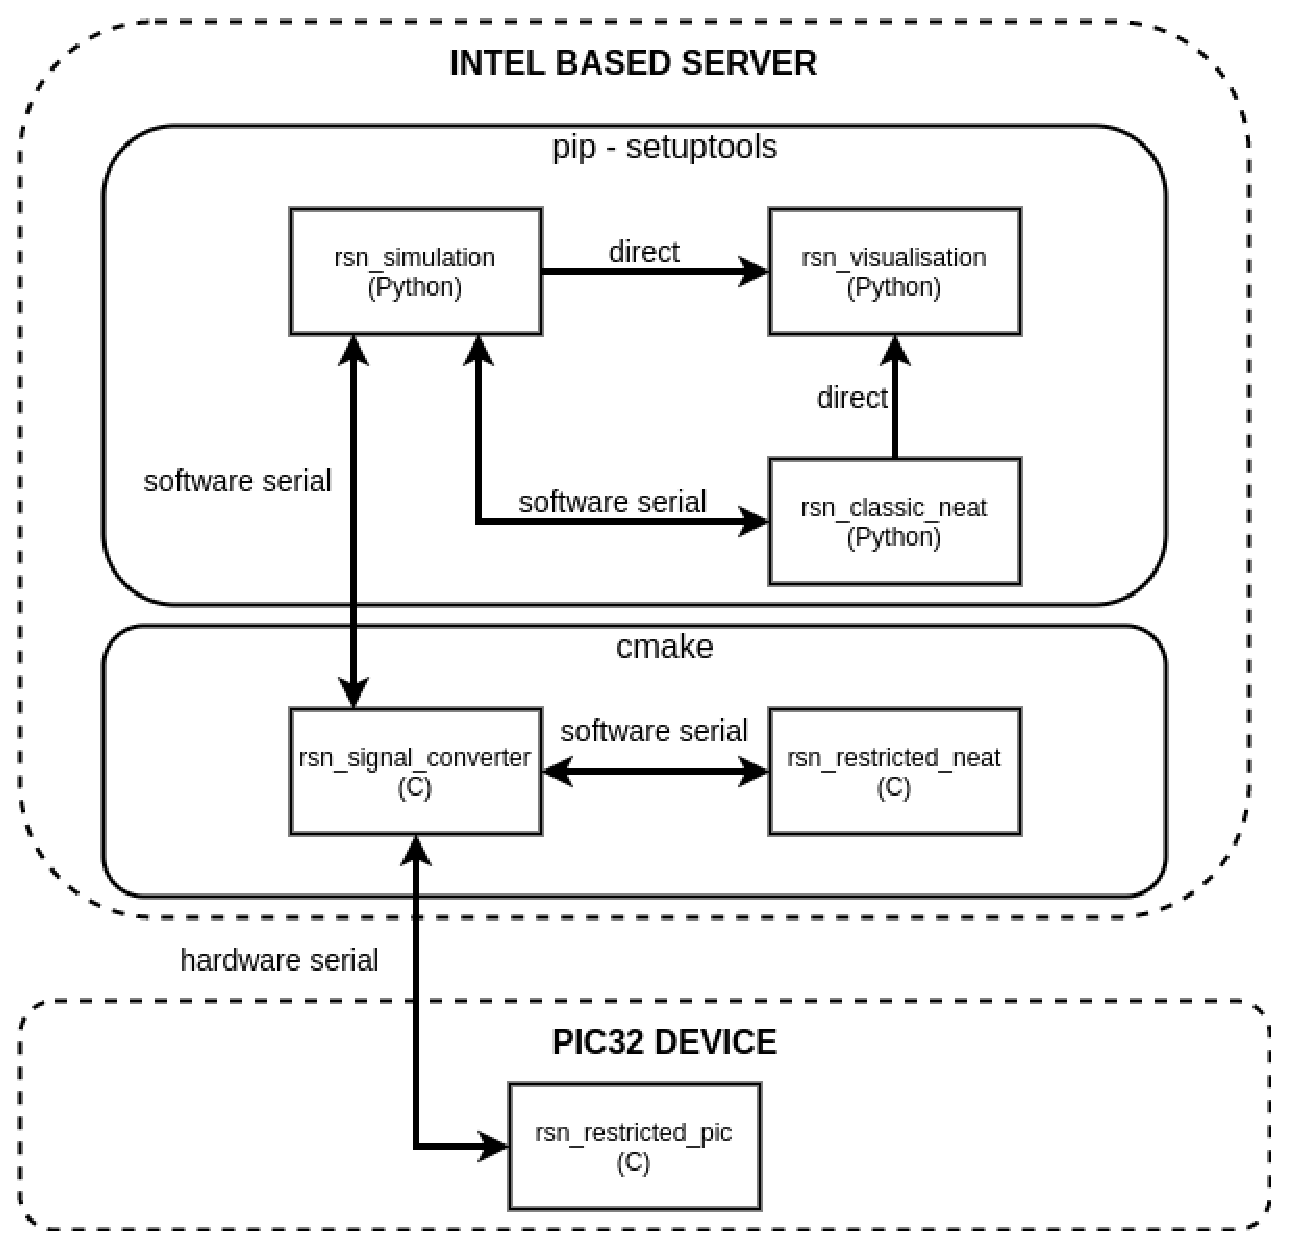
\includegraphics[width=\textwidth]{figures/experiment_arch}
	\caption{Interaction of elements within experiment architecture}
	\label{fig:experiment_arch}
\end{figure}
%==================================================================================================
\FloatBarrier
\section{AI Gym}

%--------------------------------------------------------------------------------------------------
\FloatBarrier
\subsection{Overviwe of Open AI}


%==================================================================================================
\FloatBarrier
\section{Target devices}

%==================================================================================================
\FloatBarrier
\section{Environment architecture}

%--------------------------------------------------------------------------------------------------
\FloatBarrier
\subsection{Programming languages}
Because in the target implementation of a neural network, the critical element is high 
performance and small size in memory, both for the network model and for the code itself.
Therefore, it was decided to use the C language because it provides precise control over data 
representation in memory and has minimal memory overhead for the generated code. 
During the initial phase of the experiments, a solution based on combining C with C ++ will be
used. 
The reason for this approach is the possibility of using design solutions and ready-made
libraries not available in pure C, which will ensure a much shorter prototyping period. 
The downside of this approach is the need to rewrite the final prototype from C ++ to pure C 
before installing it on the target platform.
The problem that resulted from this approach is the lack of direct integration of the created
solution with the Ai Gym environment used so far, which was written in Python and requires that 
the code using it will also be written in this language.

There are three workarounds for this issue:
\begin{enumerate}
	\item Use of a dedicated simulation environment for C / C ++.
	\item Integration between the simulation and the neural network by means of a 
		  library that enables the integration of C functions in Python.
	\item Implementation of simulations and networks as separate processes together with 
		  communication between them based on messages encoded in ASCII. 
\end{enumerate}
The first option was immediately rejected due to delays in bringing an entirely new tool to 
the design.
Several attempts have been made to integrate Python and C ++.
This approach turned out to be problematic by imposing limitations on possible solutions on
the C ++ side. 
An additional drawback was the low portability of the solution and a significant increase
in the complexity of the compilation environment.
A solution was chosen based on transferring data between two separate processes using pipes.

%--------------------------------------------------------------------------------------------------
\FloatBarrier
\subsection{Interaction between modules}

